\documentclass[12pt]{article}
\usepackage[T1]{fontenc}
\usepackage[T1]{polski}
\usepackage[utf8]{inputenc}
\usepackage{color}
\usepackage{graphicx}
\usepackage{blindtext}
\usepackage{scrextend}
\newcommand{\BibTeX}{{\sc Bib}\TeX} 
\usepackage{graphicx}
\usepackage{amsfonts}

\setlength{\textheight}{21cm}

\title{{\bf Zadanie nr 1 - Generacja sygnału i szumu}\linebreak
Cyfrowe Przetwarzanie Sygnałów}
\author{Aneta Wiśniewska, 204029 \and Hanna Paluszkiewicz, 203962}
\date{19.03.2018}

\begin{document}
\clearpage\maketitle
\thispagestyle{empty}
\newpage
\setcounter{page}{1}
\section{Cel zadania}

Celem ćwiczenia jest poznanie wybranych własności podstawowych rodzajów sygnałów. Aby to osiągnąć, trzeba napisać aplikację umożliwiającą generację jedenastu wariantów sygnałów.

\section{Wstęp teoretyczny}

\subsection{Teoria}


\addtokomafont{labelinglabel}{\sffamily}

\begin{labeling}{alligator}
\item [Sygnał] to proces zmian w czasie stanu obiektu fizycznego, bądź wielkości fizycznej.

\subitem  Rozróżniamy następujące modele matematyczne sygnałów:
\subsubitem dystrybucje
\subsubitem funkcje rzeczywiste czasu
\subsubitem funkcje zespolone

\item [Klasyfikacja sygnałów ze względu na dziedzinę okreslonosci ] ,
\subitem  Sygnały ciągłe w czasie \\
\subitem Sygnały dyskretne

\item [Klasyfikacja sygnałów ze względu na czas trwania ] ,
\subitem  Sygnały o nieskończonym czasie trwania \\
\subitem Sygnały impulsowe

\item [Klasyfikacja sygnałów ze względu na przewidywalnosć ewolucji w czasie ] ,
\subitem  Sygnały deterministyczne \\
\subitem Sygnały stochastyczne (losowe)
\end{labeling}


\subsection{Instrukcja obsługi aplikacji}
Aplikacja do generacji szumów zawiera interfejs graficzny, który służy do obsługi przez użytkownika. Wygląd został przedstawiony na poniższym rysunku.
\newpage
\begin{figure}[h!]
 \centering
 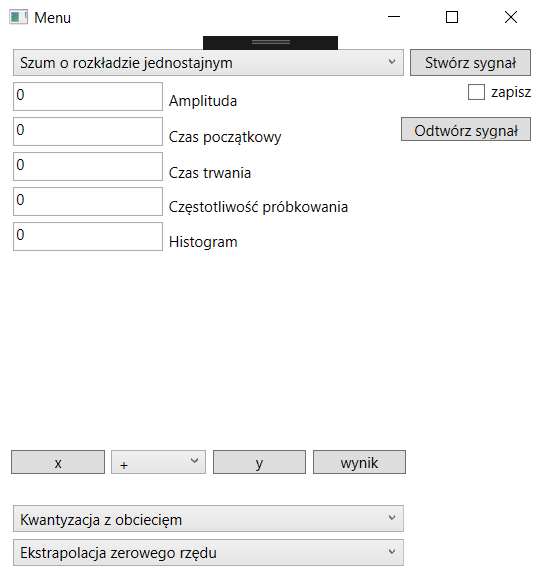
\includegraphics[width=9.3cm]{ui1.PNG}
 \vspace{-0.3cm}
 \caption{Widok główny aplikacji}
 \label{Widok_aplikacjis}
\end{figure}

Na górze okienka znajduje się wysuwana lista możliwych do generacji sygnałów. Obok znajduje się chceckbox, po zaznaczeniu którego sygnał zostanie zapisany do pliku.
Niżej jest przycisk do generacji sygnałów oraz lista parametrów wykresu. Tutaj wpisuje się dane wpływające na sygnał.
Pola umożliwiają ustawienie charakterystycznych parametrów sygnału. Na ich podstawie program wylicza wartości amplitudy sygnału w określonym czasie oraz wyświetla graficzną reprezentację sygnału w postaci wykresu funkcji amplitudy od czasu i histogramu.\\

Na dole okienka znajdują się przyciski: do odtwarzania sygnału z pliku, oraz do operacji na dwóch sygnałach. Po kliknięciu w x i y wybieramy odpowiednio pierwszy i dugi składnik działania. Między nimi można wybrać jedno z czterech działań.  Po wcisnięciu przycisku "wynik" program liczy wynik działania i wywietla jego graficzną reprezentację. 

\subsubsection{Generowanie sygnału}
Aby wygenerować sygnał użytkownik musi kliknąć w generuj sygnał.
\\Po wygenerowaniu sygnału pojawiają się dwa dodatkowe okienka aplikacji.
\begin{figure}[h!]
 \centering
 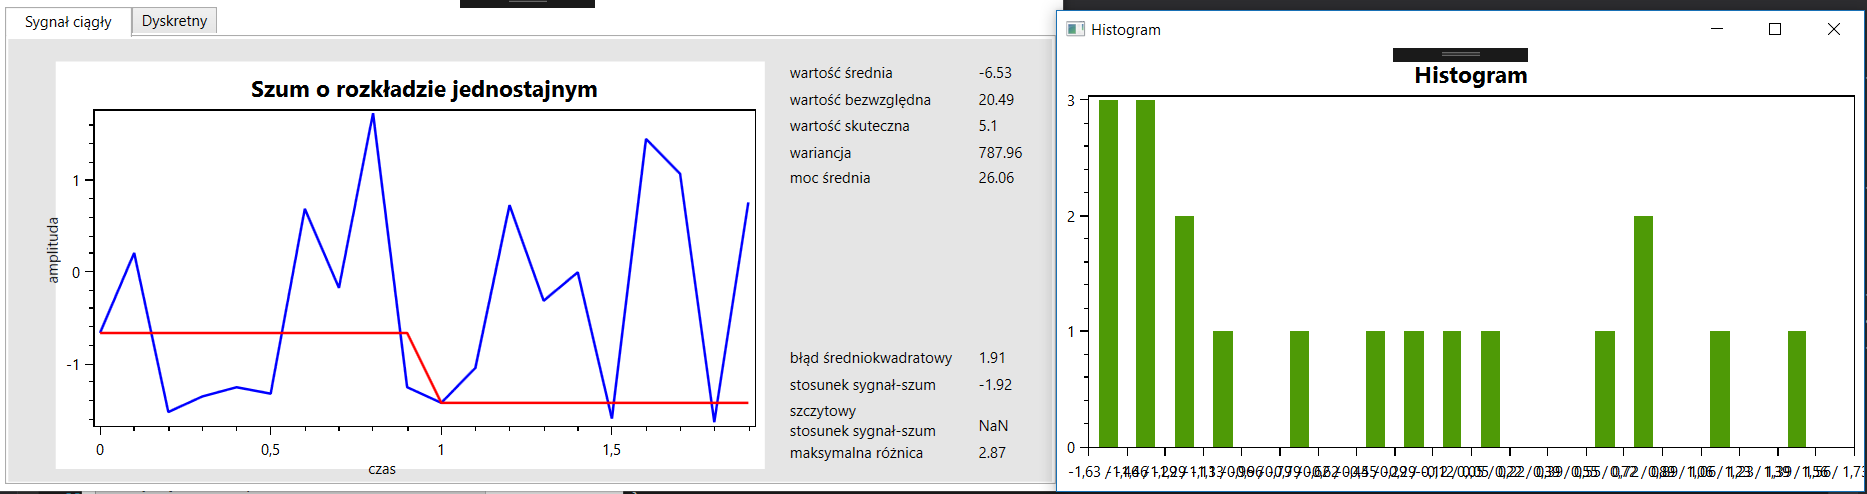
\includegraphics[width=15.3cm]{okienka.PNG}
 \vspace{-0.3cm}
 \caption{Okna po generacji sygnału}
 \label{Widok_aplikacjis}
\end{figure}
\\Jedno wyświetla histogram sygnału
\\Drugie przedstawia wykres funkcji amplitudy od czasu oraz obliczone wartości: wartość średnią, wartość średnią bezwzględną, wartość skuteczną, wariancję oraz moc średnią.

\subsubsection{Odczyt sygnału z pliku}
Oprócz generacji i zapisu do pliku, program umożliwia odczyt z pliku sygnału będącego wynikiem dyskretyzacji (bez kwantyzacji) wygenerowanego
sygnału ciągłego oraz sygnału będącego wynikiem operacji na dwóch sygnałach dyskretnych.
\\Tak jak w przypadku generacji, sygnał jest  reprezentowany graficznie w postaci histogramu i wykresu funkcji.

\subsection{Opis metod}
Opisy wszystkich metod zastosowanych do implementacji sygnałów, zostały zapisane w poszczególnych eksperymentach.

\subsection{Opis implementacji}
Aplikacja została napisana w wysokopoziomowym języku programowania - C\#. Do rysowania wykresów została wykorzystana zewnątrzna biblioteka OxyPlot. Program został napisany przy pomocy metodyki obiektowej i stosuje metody numeryczne.

\section{Eksperymenty i wyniki}

Poniżej znajdują się wszystkie przeprowadzone eksperymenty - możliwe do uzyskania w aplikacji sygnaly i wyniki. 

%%%%%%%%%%%%%%%%%%%%%%%%%%%%%%%%%%%%%%%%%%%%%%%%%%%%%%%%%%%%%%%%%%%%%%%%%%%%%%%%%%%%%%%%%%%%%%%%%%%%%%%%%%%%%%%%%
% PODROZDZIA PT. EKSPERYMENT NR 1 
%%%%%%%%%%%%%%%%%%%%%%%%%%%%%%%%%%%%%%%%%%%%%%%%%%%%%%%%%%%%%%%%%%%%%%%%%%%%%%%%%%%%%%%%%%%%%%%%%%%%%%%%%%%%%%%%%

\subsection{Eksperyment nr 1}

Eksperyment nr 1 - Szum o rozkładzie jednostajnym\\


\subsubsection{Założenia}
Amlituda generowanego sygnału przyjmuje, z jednakowym prawdopodobieństwem, losowe wartości z zakresu od <-Amax, Amax>.
Parametry: A, t1, d.
\subsubsection{Przebieg}
Do generacji synału zostały podane parametry:
\addtokomafont{labelinglabel}{\sffamily}

\begin{labeling}{szj}
\item [Amplituda (A):] 2
\item [Czas trwania (t1):] 10 s
\item [Częstotliwość próbkowania (d): ] 25 Hz
\end{labeling}

\subsubsection{Rezultat}

Rezultaty przedstawiają zamieszczone poniżej zrzuty ekranu z programu. Wartości liczbowe oraz wykres funkcji amplitudy od czasu przedstawia \ref{Wykres dla wynikw eksperymentu pierwszego}.
\begin{figure}[h!]
 \centering
 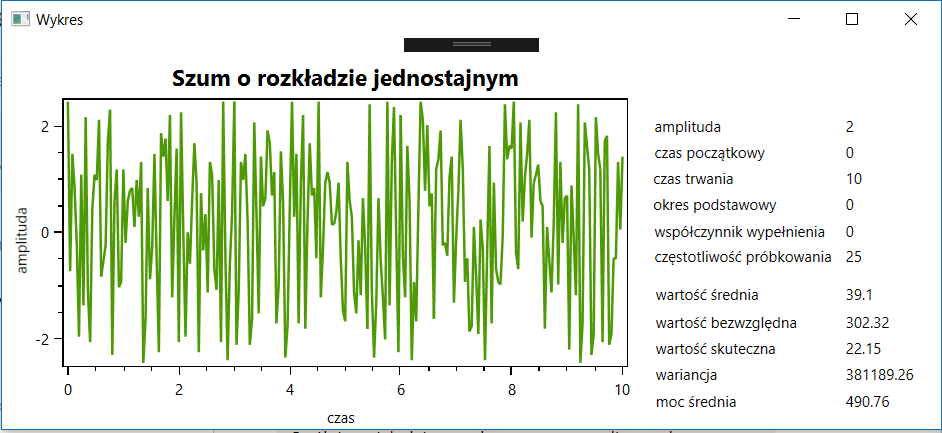
\includegraphics[width=12.3cm]{SzumRozkJedn.PNG}
 \vspace{-0.3cm}
 \caption{Wykres dla wyników eksperymentu pierwszego}
 \label{Wykres dla wynikw eksperymentu pierwszego}
\end{figure}

\newpage
Rys. \ref{Wykres dla wynikw eksperymentu pierwszego h} przedstawia histogram sygnału z opisanymi powyżej parametrami. 

\begin{figure}[h!]
 \centering
 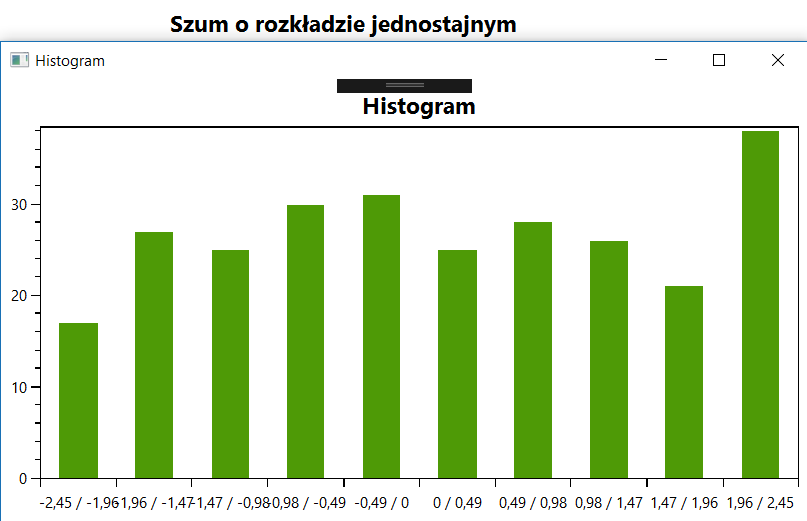
\includegraphics[width=9.3cm]{SzumRozkJednHist.PNG}
 \vspace{-0.3cm}
 \caption{Wykres dla wynikw eksperymentu pierwszego h}
 \label{Wykres dla wynikw eksperymentu pierwszego h}
\end{figure}

%%%%%%%%%%%%%%%%%%%%%%%%%%%%%%%%%%%%%%%%%%%%%%%%%%%%%%%%%%%%%%%%%%%%%%%%%%%%%%%%%%%%%%%%%%%%%%%%%%%%%%%%%%%%%%%%%
% PODROZDZIA PT. EKSPERYMENT NR2 
%%%%%%%%%%%%%%%%%%%%%%%%%%%%%%%%%%%%%%%%%%%%%%%%%%%%%%%%%%%%%%%%%%%%%%%%%%%%%%%%%%%%%%%%%%%%%%%%%%%%%%%%%%%%%%%%%

\subsection{Eksperyment nr 2}

Eksperyment nr 2  - Szum gaussowski

\subsubsection{Założenia}
W szumie gaussowskim amplituda przyjmuje losowe wartości. Rozkład gęstości prawdopodobieństwa tych wartości jest rozkładem normalnym,czyli funkcja gęstości rozkładu zmiennej losowe jprzedstawia wzór:

\begin{figure}[h!]
 \centering
 \includegraphics[width=4.3cm]{GaussWzor.PNG}
 \vspace{-0.3cm}
 \label{gw}
\end{figure}

gdzie:
mi - średnia (należy przyjąć wartość 0);
gamma - odchylenie standardowe (należy przyjąć wartość 1).
Generując sygnał należy posłużyć się generatorem liczb losowych o rozkładzie
normalnym.
Parametry: A, t1, d.

\subsubsection{Przebieg}
Do generacji synału zostały podane parametry:
\addtokomafont{labelinglabel}{\sffamily}

\begin{labeling}{szj}
\item [Amplituda (A):] 2
\item [Czas trwania (t1):] 10 s
\item [Częstotliwość próbkowania (d): ] 25 Hz
\end{labeling}
\subsubsection{Rezultat}

Rezultaty przedstawiają zamieszczone poniżej zrzuty ekranu z programu. Wartości liczbowe oraz wykres funkcji amplitudy od czasu przedstawia \ref{Histogram dla wyników eksperymentu drugiego}.
\begin{figure}[h!]
 \centering
 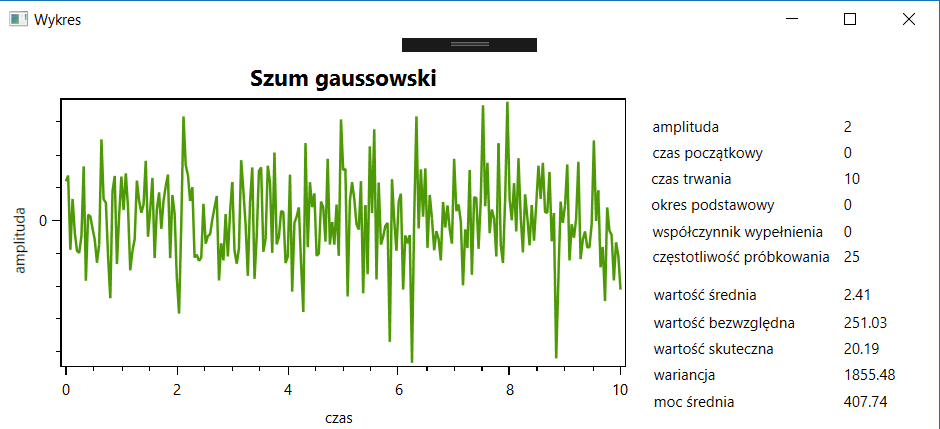
\includegraphics[width=12.3cm]{szumGauss.PNG}
 \vspace{-0.3cm}
 \caption{Wykres dla wyników eksperymentu drugiego}
 \label{Wykres dla wyników eksperymentu drugiego}
\end{figure}
\newpage
Rys. \ref{Wykres dla wynikw eksperymentu pierwszego h} przedstawia histogram sygnału z opisanymi powyżej parametrami. 
\begin{figure}[h!]
 \centering
 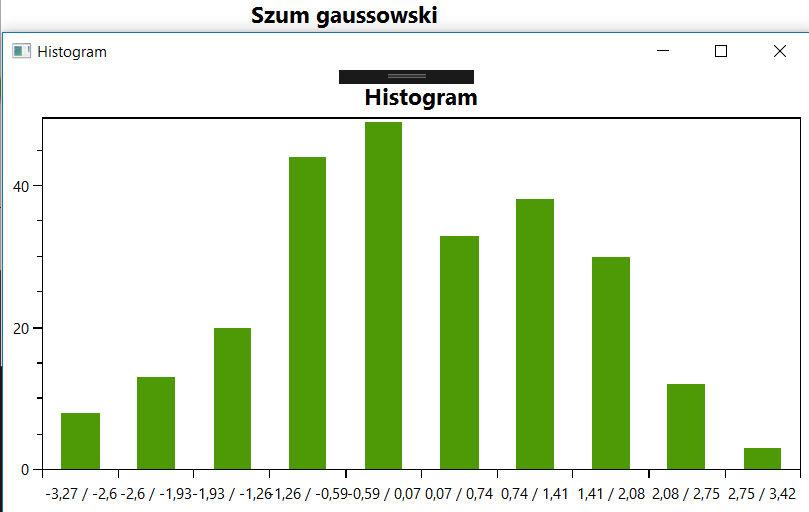
\includegraphics[width=9.3cm]{szumGaussHist.PNG}
 \vspace{-0.3cm}
 \caption{Histogram dla wyników eksperymentu drugiego}
 \label{Histogram dla wyników eksperymentu drugiego}
\end{figure}

%%%%%%%%%%%%%%%%%%%%%%%%%%%%%%%%%%%%%%%%%%%%%%%%%%%%%%%%%%%%%%%%%%%%%%%%%%%%%%%%%%%%%%%%%%%%%%%%%%%%%%%%%%%%%%%%%
% PODROZDZIA PT. EKSPERYMENT NR 3 
%%%%%%%%%%%%%%%%%%%%%%%%%%%%%%%%%%%%%%%%%%%%%%%%%%%%%%%%%%%%%%%%%%%%%%%%%%%%%%%%%%%%%%%%%%%%%%%%%%%%%%%%%%%%%%%%%

\subsection{Eksperyment nr 3}

Eksperyment nr 3 Sygnał sinusoidalny

\subsubsection{Założenia}
Sygnał opisuje wzór:

\begin{figure}[h!]
 \centering
 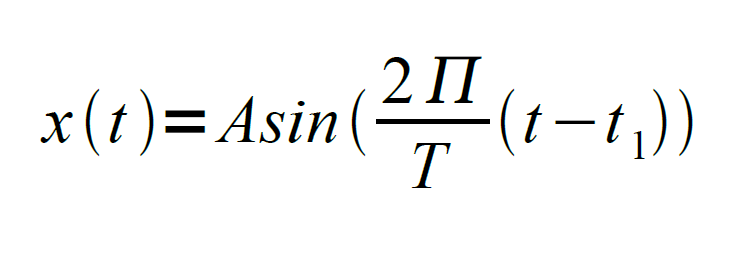
\includegraphics[width=4.3cm]{SinWzor.PNG}
 \vspace{-0.3cm}
 \label{gw}
\end{figure}

Parametry: A, T t1, d.


\subsubsection{Przebieg}
Do generacji synału zostały podane parametry:
\addtokomafont{labelinglabel}{\sffamily}

\begin{labeling}{szj}
\item [Amplituda (A):] 3
\item [Czas trwania (t1):] 20 s
\item [Częstotliwość próbkowania (d): ] 40 Hz
\end{labeling}


\subsubsection{Rezultat}

Rezultaty przedstawiają zamieszczone poniżej zrzuty ekranu z programu. Wartości liczbowe oraz wykres funkcji amplitudy od czasu przedstawia \ref{Wykres dla wyników eksperymentu trzeciego}.
\begin{figure}[h!]
 \centering
 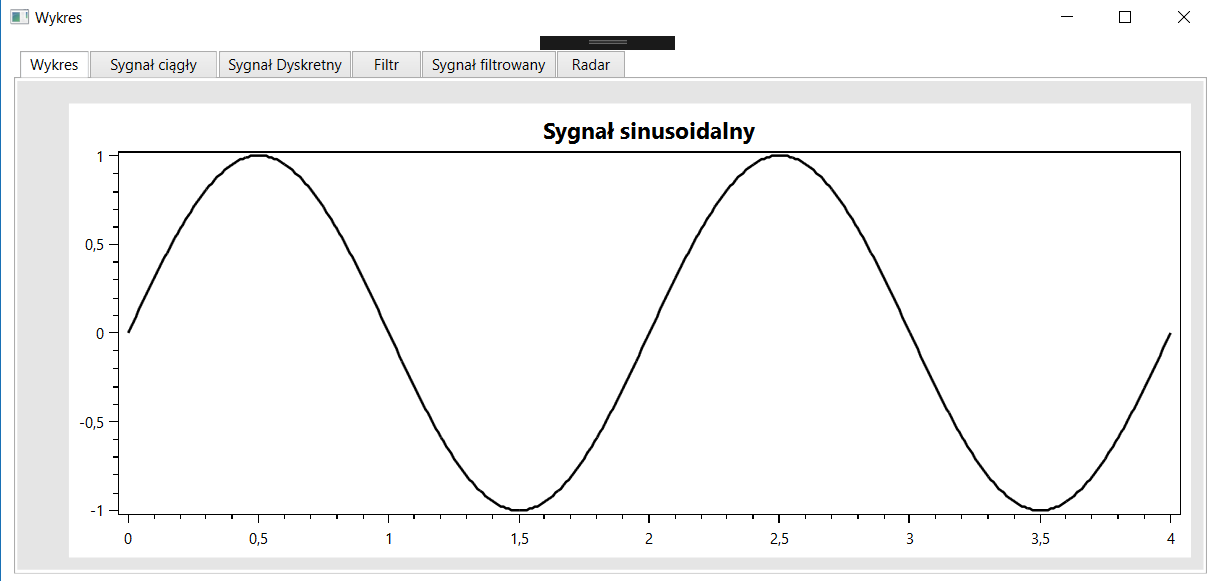
\includegraphics[width=12.3cm]{Sin.PNG}
 \vspace{-0.3cm}
 \caption{Wykres dla wyników eksperymentu trzeciego}
 \label{Wykres dla wyników eksperymentu trzeciego}
\end{figure}

\newpage
Rys. \ref{Histogram dla wyników eksperymentu trzeciego} przedstawia histogram sygnału z opisanymi powyżej parametrami. 
\begin{figure}[h!]
 \centering
 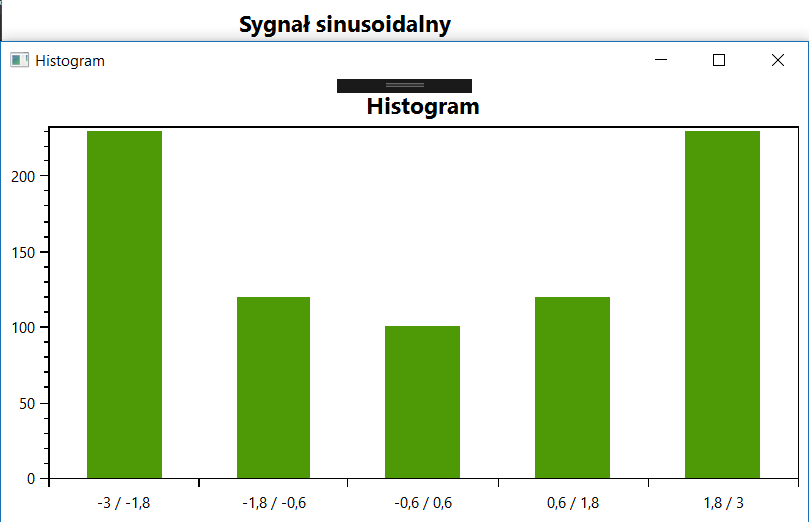
\includegraphics[width=9.3cm]{SinHist.PNG}
 \vspace{-0.3cm}
 \caption{Histogram dla wyników eksperymentu trzeciego}
 \label{Histogram dla wyników eksperymentu trzeciego}
\end{figure}

%%%%%%%%%%%%%%%%%%%%%%%%%%%%%%%%%%%%%%%%%%%%%%%%%%%%%%%%%%%%%%%%%%%%%%%%%%%%%%%%%%%%%%%%%%%%%%%%%%%%%%%%%%%%%%%%%
% PODROZDZIA PT. EKSPERYMENT NR4 
%%%%%%%%%%%%%%%%%%%%%%%%%%%%%%%%%%%%%%%%%%%%%%%%%%%%%%%%%%%%%%%%%%%%%%%%%%%%%%%%%%%%%%%%%%%%%%%%%%%%%%%%%%%%%%%%%

\subsection{Eksperyment nr 4}

Eksperyment nr 4 - Sygnał sinusoidalny wyprostowany jednopołówkowo\\

\subsubsection{Założenia}
Sygnał opisuje wzór:
\begin{figure}[h!]
 \centering
 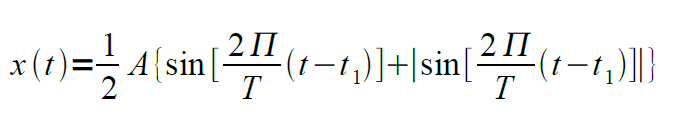
\includegraphics[width=9.3cm]{SinJedPWzor.PNG}
 \vspace{-0.3cm}
 \label{gw}
\end{figure}
\newpage
Parametry: A, T t1, d.

\subsubsection{Przebieg}
Do generacji synału zostały podane parametry:
\addtokomafont{labelinglabel}{\sffamily}

\begin{labeling}{szj}
\item [Amplituda (A):] 2
\item [Czas trwania (t1):] 10 s
\item [Częstotliwość próbkowania (d): ] 25 Hz
\end{labeling}

\subsubsection{Rezultat}

Rezultaty przedstawiają zamieszczone poniżej zrzuty ekranu z programu. Wartości liczbowe oraz wykres funkcji amplitudy od czasu przedstawia \ref{Wykres dla wyników eksperymentu czwartego}.
\begin{figure}[h!]
 \centering
 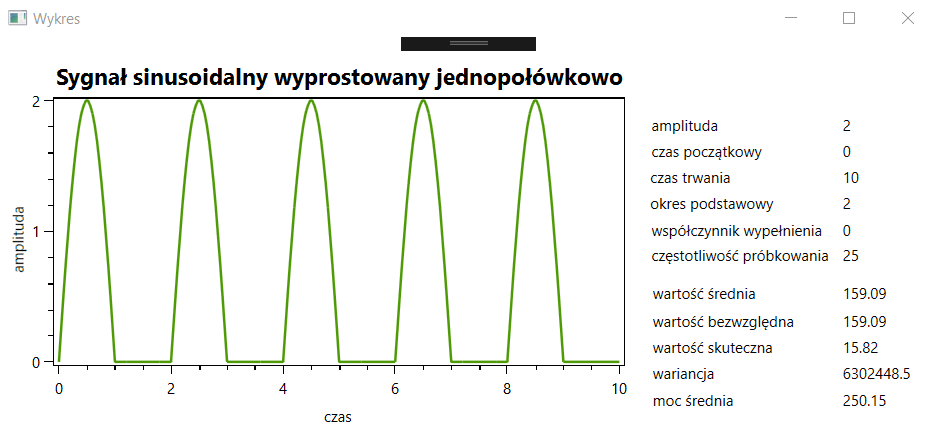
\includegraphics[width=12.3cm]{SinJednoP.PNG}
 \vspace{-0.3cm}
 \caption{Wykres dla wyników eksperymentu czwartego}
 \label{Wykres dla wyników eksperymentu czwartego}
\end{figure}

\newpage
Rys. \ref{Histogram dla wyników eksperymentu czwartego} przedstawia histogram sygnału z opisanymi powyżej parametrami. 
\begin{figure}[h!]
 \centering
 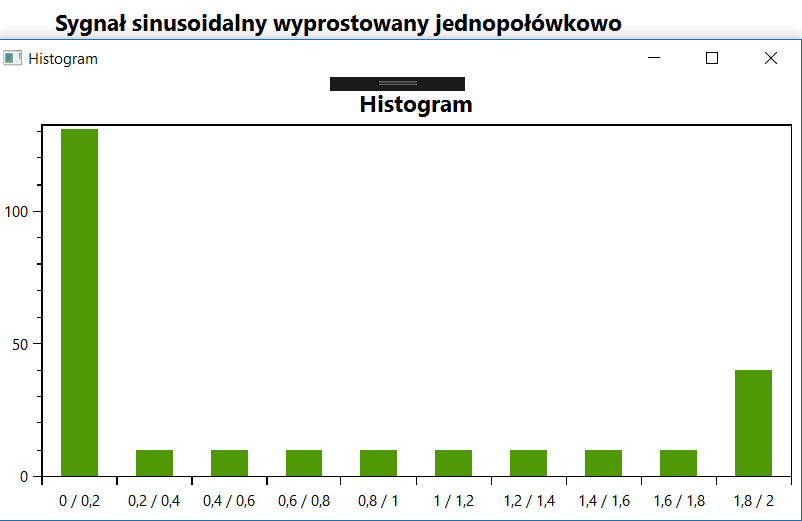
\includegraphics[width=9.3cm]{SinJednoPHist.PNG}
 \vspace{-0.3cm}
 \caption{Histogram dla wyników eksperymentu czwartego}
 \label{Histogram dla wyników eksperymentu czwartego}
\end{figure}

\subsection{Eksperyment nr 5}

\subsubsection{Założenia}
Sygnał opisuje wzór:
\begin{figure}[h!]
 \centering
 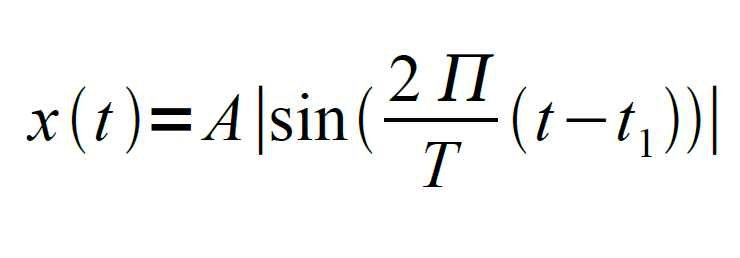
\includegraphics[width=4.3cm]{SinDwuPWzor.PNG}
 \vspace{-0.3cm}
 \label{gw}
\end{figure}
\newpage
Parametry: A, T t1, d.

\subsubsection{Przebieg}
Do generacji synału zostały podane parametry:
\addtokomafont{labelinglabel}{\sffamily}

\begin{labeling}{szj}
\item [Amplituda (A):] 2
\item [Czas trwania (t1):] 10 s
\item [Częstotliwość próbkowania (d): ] 25 Hz
\end{labeling}

\subsubsection{Rezultat}
Rezultaty przedstawiają zamieszczone poniżej zrzuty ekranu z programu. Wartości liczbowe oraz wykres funkcji amplitudy od czasu przedstawia \ref{Wykres dla wyników eksperymentu piątego}.
\begin{figure}[h!]
 \centering
 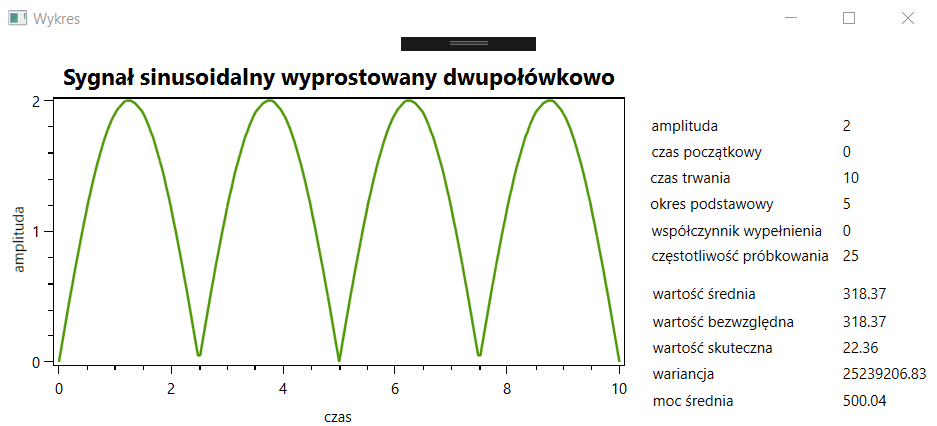
\includegraphics[width=12.3cm]{SinDwuP.PNG}
 \vspace{-0.3cm}
 \caption{Wykres dla wyników eksperymentu piątego}
 \label{Wykres dla wyników eksperymentu piątego}
\end{figure}

\newpage
Rys. \ref{Histogram dla wyników eksperymentu piątego} przedstawia histogram sygnału z opisanymi powyżej parametrami. 
\begin{figure}[h!]
 \centering
 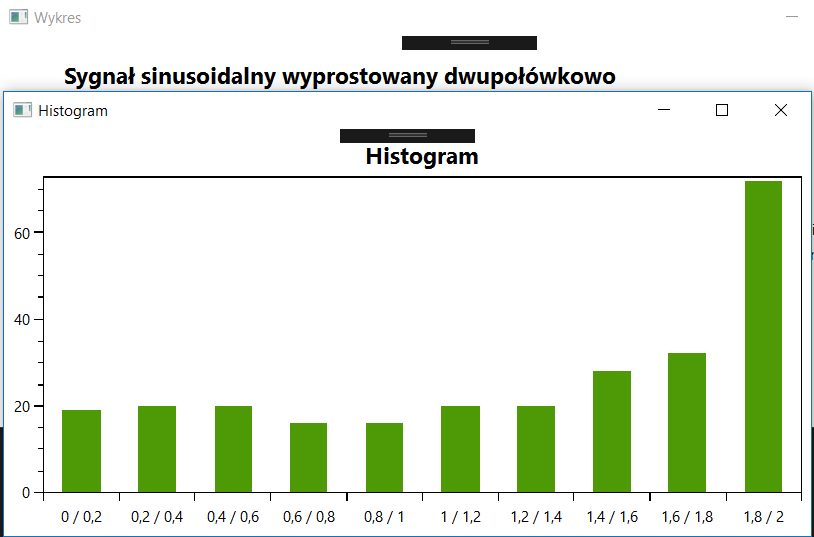
\includegraphics[width=9.3cm]{SinDwuPHist.PNG}
 \vspace{-0.3cm}
 \caption{Histogram dla wyników eksperymentu piątego}
 \label{Histogram dla wyników eksperymentu piątego}
\end{figure}

\subsection{Eksperyment nr 6}

Eksperyment nr 6 - Sygnał prostokątny

\subsubsection{Założenia}
Sygnał można opisać wzorem:
\begin{figure}[h!]
 \centering
 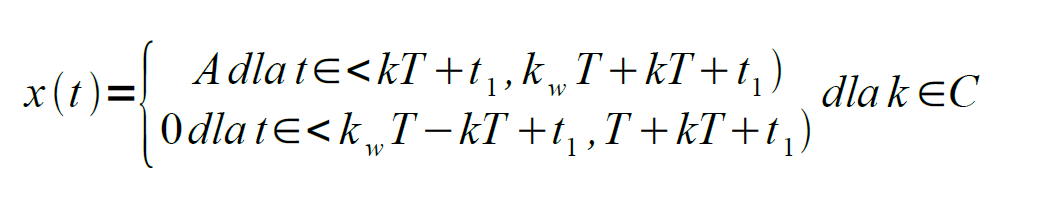
\includegraphics[width=9.3cm]{KwadWzor.PNG}
 \vspace{-0.3cm}
 \label{gw}
\end{figure}
\newpage
Parametry: A, T t1, d, kw.\\
Ze względu na problemy implementacyjne nie został zastosowany w programie. Zamiast niego została zaimplementowana autorska metoda.
\subsubsection{Przebieg}
Do generacji synału zostały podane parametry:
\addtokomafont{labelinglabel}{\sffamily}

\begin{labeling}{szj}
\item [Amplituda (A):] 2
\item [Czas trwania (t1):] 100 s
\item [okres podstawowy (T):] 50 s
\item [współczynnik wypełnienia (k):] 0.5
\item [Częstotliwość próbkowania (d): ] 25 Hz
\end{labeling}

\subsubsection{Rezultat}
Rezultaty przedstawiają zamieszczone poniżej zrzuty ekranu z programu. Wartości liczbowe oraz wykres funkcji amplitudy od czasu przedstawia \ref{Wykres dla wyników eksperymentu szóstego}.

\begin{figure}[h!]
 \centering
 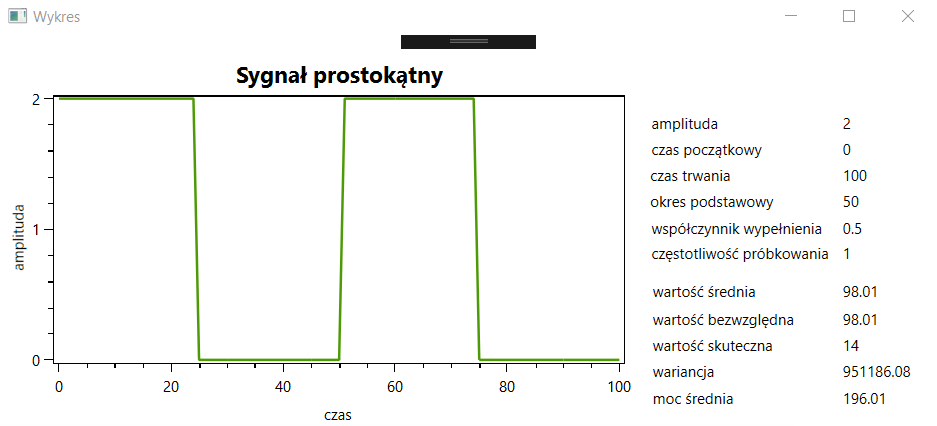
\includegraphics[width=12.3cm]{SygProst.PNG}
 \vspace{-0.3cm}
 \caption{Wykres dla wyników eksperymentu szóstego}
 \label{Wykres dla wyników eksperymentu szóstego}
\end{figure}
\newpage
Rys. \ref{Histogram dla wyników eksperymentu szóstego} przedstawia histogram sygnału z opisanymi powyżej parametrami. 
\begin{figure}[h!]
 \centering
 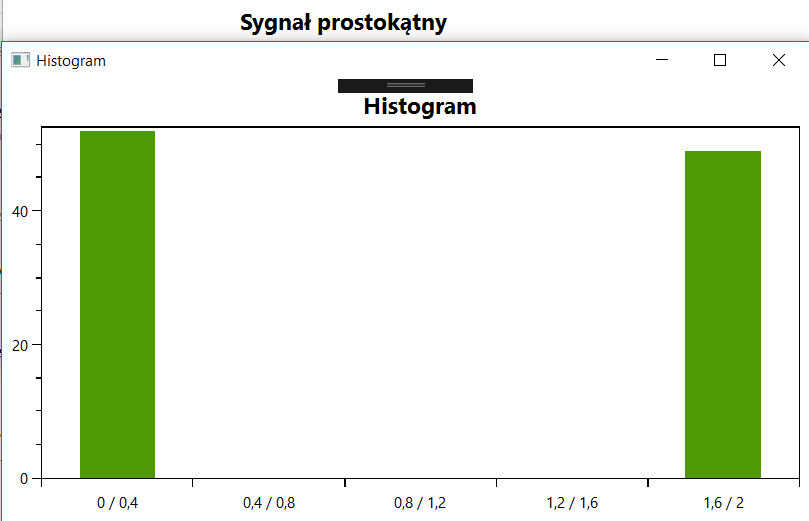
\includegraphics[width=9.3cm]{SygProstHist.PNG}
 \vspace{-0.3cm}
 \caption{Histogram dla wyników eksperymentu szóstego}
 \label{Histogram dla wyników eksperymentu szóstego}
\end{figure}

\subsection{Eksperyment nr 7}

Eksperyment nr 7 - Sygnał prostokątny symetryczny

\subsubsection{Założenia}
Sygnał można opisać wzorem:
\begin{figure}[h!]
 \centering
 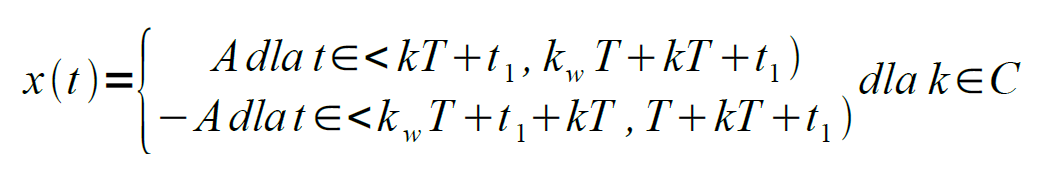
\includegraphics[width=9.3cm]{KwadWzorSym.PNG}
 \vspace{-0.3cm}
 \label{gw}
\end{figure}
\newpage
Parametry: A, T t1, d, kw.\\
Ze względu na problemy implementacyjne nie został zastosowany w programie. Zamiast niego została zaimplementowana autorska metoda.

\subsubsection{Przebieg}
Do generacji synału zostały podane parametry:
\addtokomafont{labelinglabel}{\sffamily}

\begin{labeling}{szj}
\item [Amplituda (A):] 2
\item [Czas trwania (t1):] 100 s
\item [okres podstawowy (T):] 50 s
\item [współczynnik wypełnienia (k):] 0.5
\item [Częstotliwość próbkowania (d): ] 25 Hz
\end{labeling}

\subsubsection{Rezultat}
Rezultaty przedstawiają zamieszczone poniżej zrzuty ekranu z programu. Wartości liczbowe oraz wykres funkcji amplitudy od czasu przedstawia \ref{Wykres dla wyników eksperymentu siódmego}.
\begin{figure}[h!]
 \centering
 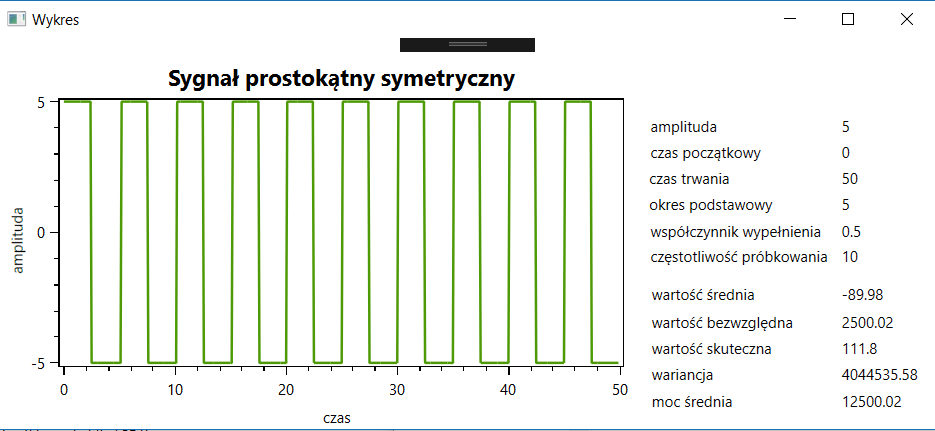
\includegraphics[width=12.3cm]{SygProstSym.PNG}
 \vspace{-0.3cm}
 \caption{Wykres dla wyników eksperymentu siódmego}
 \label{Wykres dla wyników eksperymentu siódmego}
\end{figure}

\newpage
Rys. \ref{Histogram dla wyników eksperymentu szóstego} przedstawia histogram sygnału z opisanymi powyżej parametrami. 
\begin{figure}[h!]
 \centering
 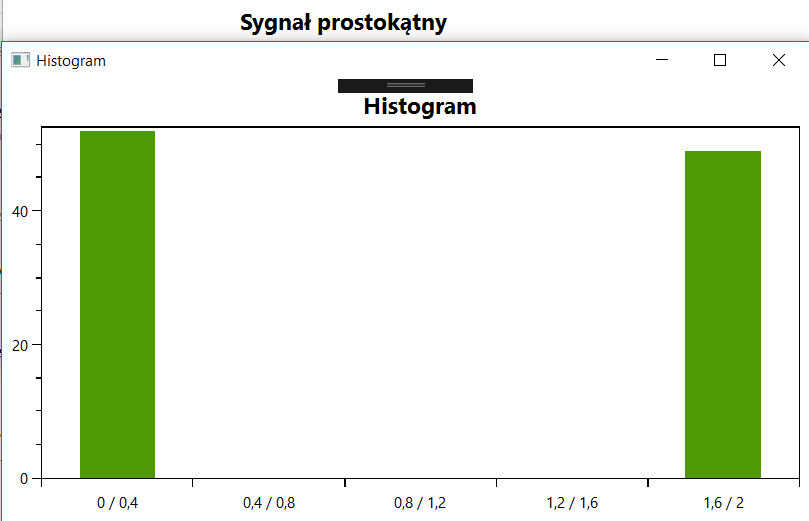
\includegraphics[width=9.3cm]{SygProstHist.PNG}
 \vspace{-0.3cm}
 \caption{Histogram dla wyników eksperymentu szóstego}
 \label{Histogram dla wyników eksperymentu szóstego}
\end{figure}

\subsection{Eksperyment nr 8}

Eksperyment nr 8 - Sygnał trójkątny

\subsubsection{Założenia}
Sygnał opisuje wzór:
\begin{figure}[h!]
 \centering
 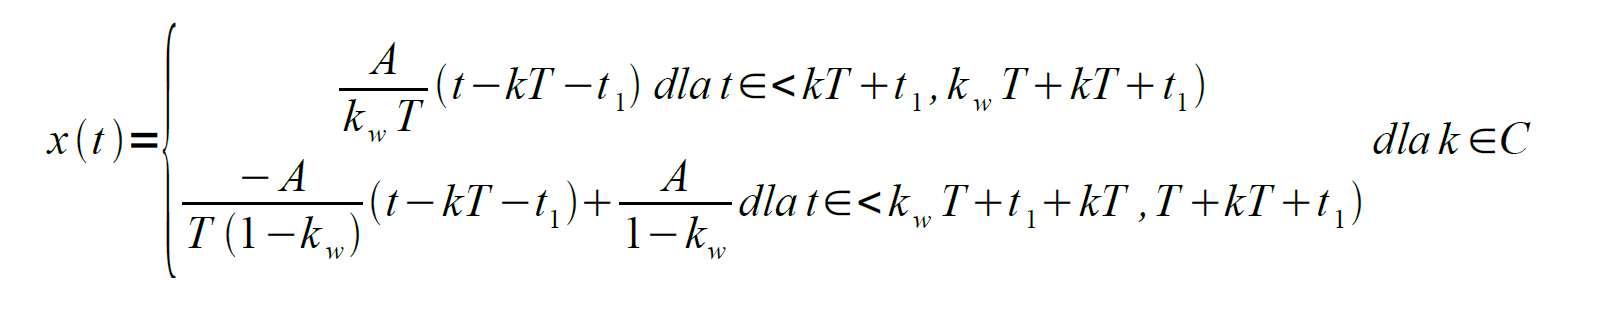
\includegraphics[width=9.3cm]{TrojWzor.PNG}
 \vspace{-0.3cm}
 \label{gw}
\end{figure}
\newpage
Parametry: A, T t1, d, kw.
\\Ze względu na problemy implementacyjne nie został zastosowany w programie. Zamiast niego została zaimplementowana autorska metoda.
\subsubsection{Przebieg}
Do generacji synału zostały podane parametry:
\addtokomafont{labelinglabel}{\sffamily}

\begin{labeling}{szj}
\item [Amplituda (A):] 2
\item [Czas trwania (t1):] 100 s
\item [okres podstawowy (T):] 50 s
\item [współczynnik wypełnienia (k):] 0.5
\item [Częstotliwość próbkowania (d): ] 25 Hz
\end{labeling}

\subsubsection{Rezultat}
Rezultaty przedstawiają zamieszczone poniżej zrzuty ekranu z programu. Wartości liczbowe oraz wykres funkcji amplitudy od czasu przedstawia \ref{Wykres dla wyników eksperymentu ósmego}.

\begin{figure}[h!]
 \centering
 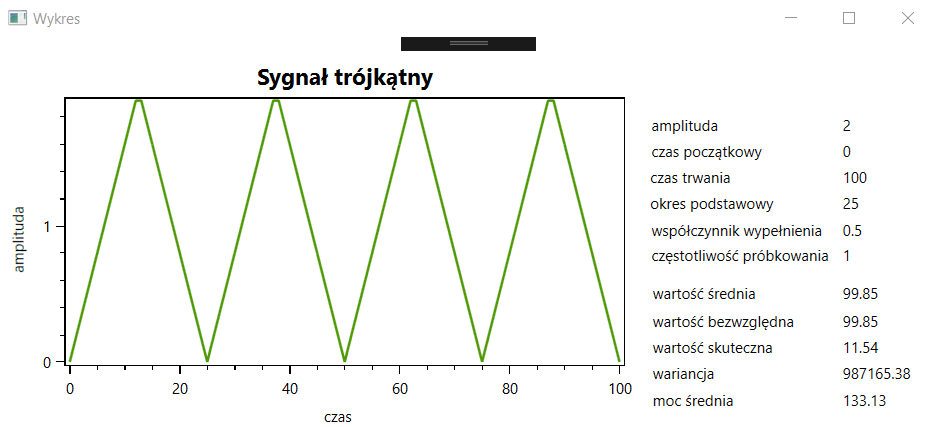
\includegraphics[width=12.3cm]{SygTroj.PNG}
 \vspace{-0.3cm}
 \caption{Wykres dla wyników eksperymentu ósmego}
 \label{Wykres dla wyników eksperymentu ósmego}
\end{figure}
\newpage
Rys. \ref{Histogram dla wyników eksperymentu ósmego} przedstawia histogram sygnału z opisanymi powyżej parametrami. 
\begin{figure}[h!]
 \centering
 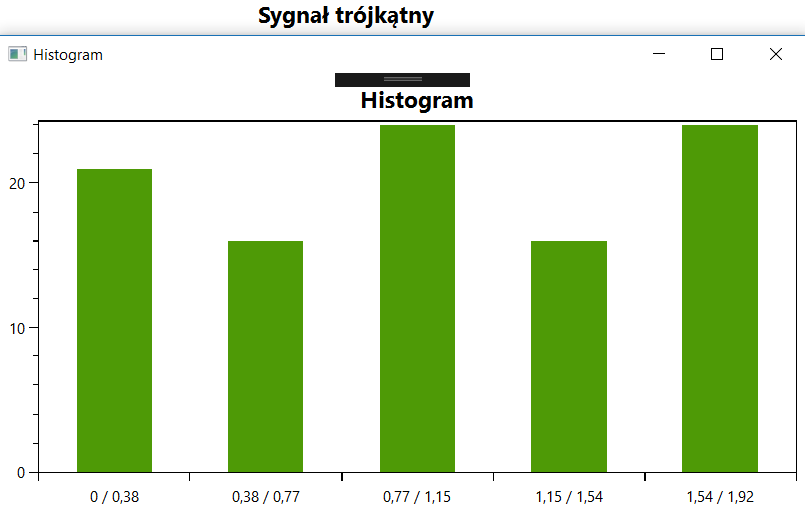
\includegraphics[width=9.3cm]{SygTrojHist.PNG}
 \vspace{-0.3cm}
 \caption{Histogram dla wyników eksperymentu ósmego}
 \label{Histogram dla wyników eksperymentu ósmego}
\end{figure}

\subsection{Eksperyment nr 9}

Eksperyment nr 9 - Skok jednostkowy

\subsubsection{Założenia}
Sygnał opisuje wzór:
\begin{figure}[h!]
 \centering
 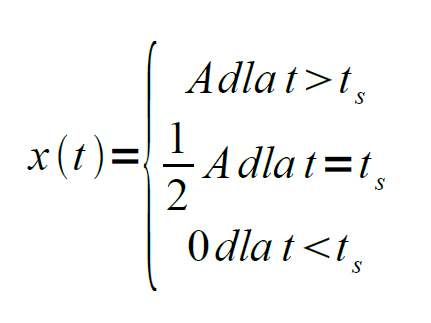
\includegraphics[width=4.3cm]{SkowJWzor.PNG}
 \vspace{-0.3cm}
 \label{gw}
\end{figure}
\newpage
Parametry: A, T t1, d, kw.

\subsubsection{Przebieg}
Do generacji synału zostały podane parametry:
\addtokomafont{labelinglabel}{\sffamily}

\begin{labeling}{szj}
\item [Amplituda (A):] 2
\item [Czas trwania (t1):] 100 s
\item [okres podstawowy (T):] 50 s
\item [współczynnik wypełnienia (k):] 0.5
\item [Częstotliwość próbkowania (d): ] 25 Hz
\end{labeling}

\subsubsection{Rezultat}
Rezultaty przedstawiają zamieszczone poniżej zrzuty ekranu z programu. Wartości liczbowe oraz wykres funkcji amplitudy od czasu przedstawia \ref{Wykres dla wyników eksperymentu dziewiątego}.

\begin{figure}[h!]
 \centering
 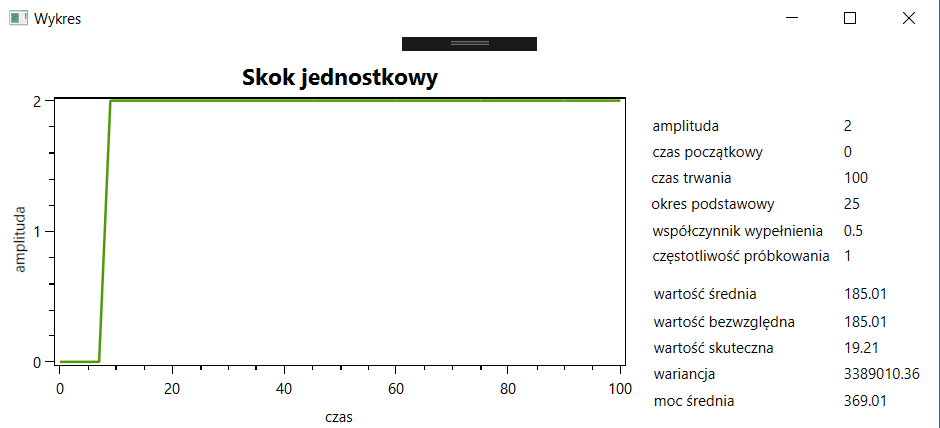
\includegraphics[width=12.3cm]{SkokJed.PNG}
 \vspace{-0.3cm}
 \caption{Wykres dla wyników eksperymentu dziewiątego}
 \label{Wykres dla wyników eksperymentu dziewiątego}
\end{figure}
\newpage
Rys. \ref{Histogram dla wyników eksperymentu dziewiątego} przedstawia histogram sygnału z opisanymi powyżej parametrami. 
\begin{figure}[h!]
 \centering
 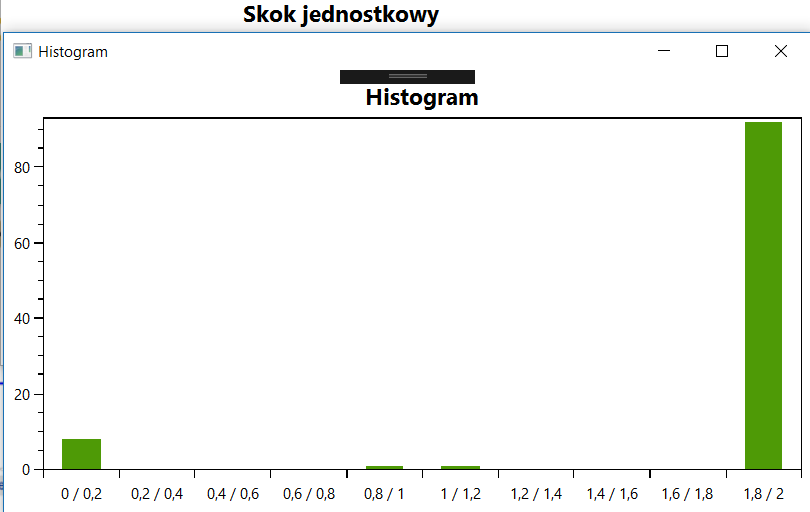
\includegraphics[width=9.3cm]{SkokJedHist.PNG}
 \vspace{-0.3cm}
 \caption{Histogram dla wyników eksperymentu dziewiątego}
 \label{Histogram dla wyników eksperymentu dziewiątego}
\end{figure}

\subsection{Eksperyment nr 10}

Eksperyment nr 10 - Impuls jednostkowy

\subsubsection{Założenia}
Sygnał opisuje wzór:
\begin{figure}[h!]
 \centering
 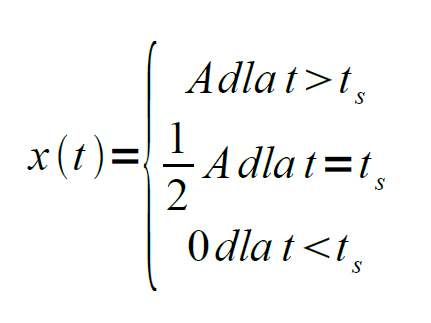
\includegraphics[width=4.3cm]{SkowJWzor.PNG}
 \vspace{-0.3cm}
 \label{gw}
\end{figure}
\newpage
Parametry: A, T t1, d, kw.

\subsubsection{Przebieg}
Do generacji synału zostały podane parametry:
\addtokomafont{labelinglabel}{\sffamily}

\begin{labeling}{szj}
\item [Amplituda (A):] 2
\item [Czas trwania (t1):] 100 s
\item [okres podstawowy (T):] 50 s
\item [współczynnik wypełnienia (k):] 0.5
\item [Częstotliwość próbkowania (d): ] 25 Hz
\end{labeling}

\subsubsection{Rezultat}
Rezultaty przedstawiają zamieszczone poniżej zrzuty ekranu z programu. Wartości liczbowe oraz wykres funkcji amplitudy od czasu przedstawia \ref{Wykres dla wyników eksperymentu dziesiątego}.

\begin{figure}[h!]
 \centering
 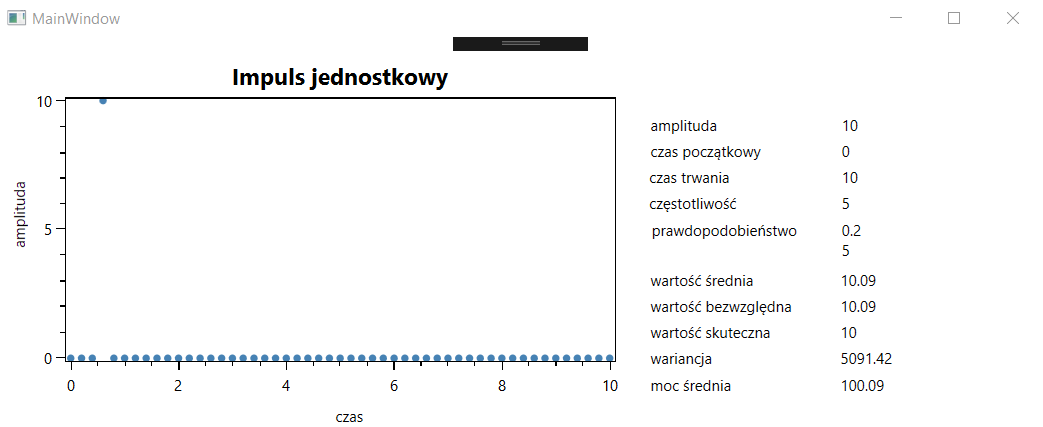
\includegraphics[width=12.3cm]{ImpulsJed.PNG}
 \vspace{-0.3cm}
 \caption{Wykres dla wyników eksperymentu dziesiątego}
 \label{Wykres dla wyników eksperymentu dziesiątego}
\end{figure}
\newpage
\begin{figure}[h!]
 \centering
 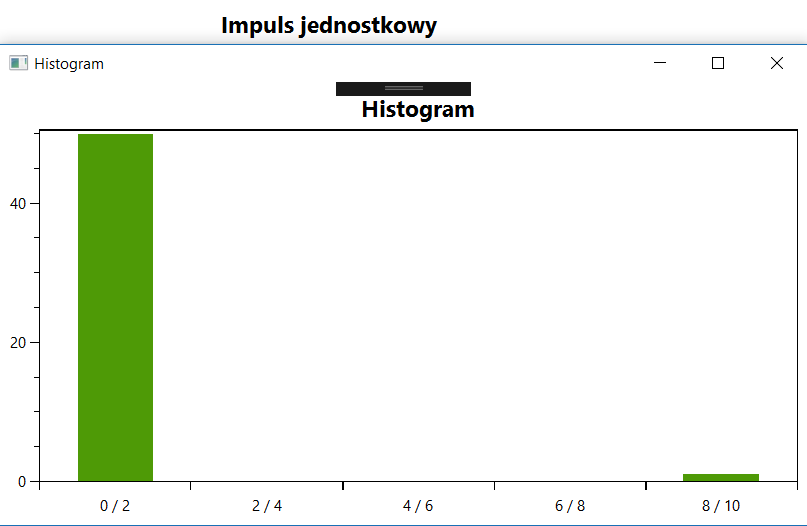
\includegraphics[width=9.3cm]{ImpulsJedHist.PNG}
 \vspace{-0.3cm}
 \caption{Histogram dla wyników eksperymentu dziesiątego}
 \label{Histogram dla wyników eksperymentu dziesiątego}
\end{figure}

\subsection{Eksperyment nr 11}

Eksperyment nr 11 - Szum impulsowy
\subsubsection{Założenia}
Szum impulsowy jest to sygnałem dyskretnym, którego amplituda przyjmuje wartość 0 oraz wartość A różną od zera.
Parametry: A, t1, d, f, p gdzie p jest prawdopodobieństwem wystąpienia wartości A.

\subsubsection{Przebieg}
Do generacji synału zostały podane parametry:
\addtokomafont{labelinglabel}{\sffamily}

\begin{labeling}{szj}
\item [Amplituda (A):] 2
\item [Czas trwania (t1):] 100 s
\item [okres podstawowy (T):] 50 s
\item [współczynnik wypełnienia (k):] 0.5
\item [Częstotliwość próbkowania (d): ] 25 Hz
\end{labeling}

\subsubsection{Rezultat}
Rezultaty przedstawiają zamieszczone poniżej zrzuty ekranu z programu. Wartości liczbowe oraz wykres funkcji amplitudy od czasu przedstawia \ref{Wykres dla wyników eksperymentu dziesiątego}.
\begin{figure}[h!]
 \centering
 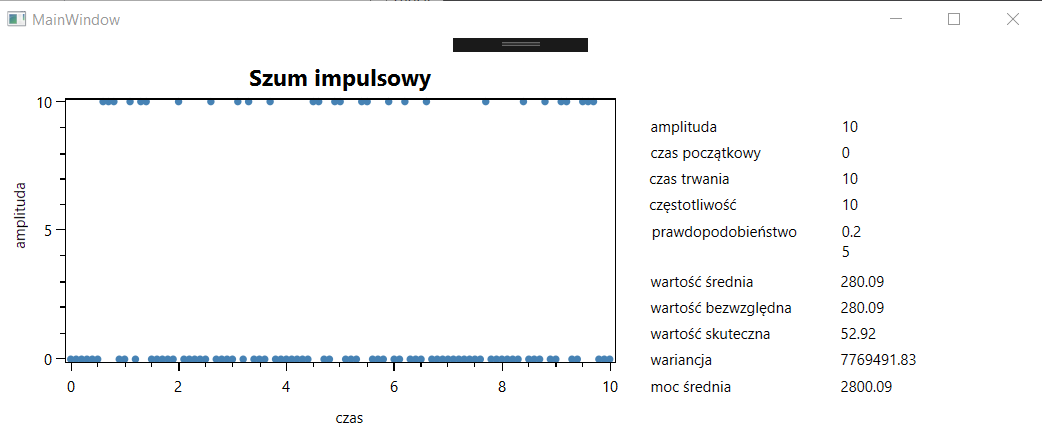
\includegraphics[width=12.3cm]{SzumImp.PNG}
 \vspace{-0.3cm}
 \caption{Wykres dla wynikw eksperymentu pierwszego}
 \label{rysunek do eksperymentu pierwszego}
\end{figure}
\newpage
\begin{figure}[h!]
 \centering
 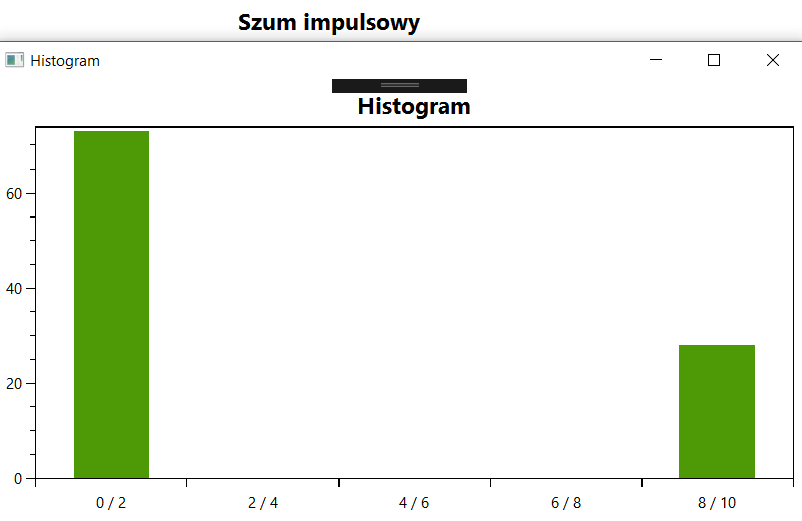
\includegraphics[width=9.3cm]{SzumImpHist.PNG}
 \vspace{-0.3cm}
 \caption{Wykres dla wynikw eksperymentu pierwszego}
 \label{rysunek do eksperymentu pierwszego}
\end{figure}


\subsection{Eksperyment nr 12}

Eksperyment nr 12 - dodawanie sygnałów

\subsubsection{Założenia}
Aby wykonać operacje na sygnałach, muszą zgadzać się ich parametry.

\subsubsection{Przebieg}
Do generacji sumy synałów zostały wybrane sygnał sinusoidalny i szum o rozkładzie normalnym o jednakowych podanych parametrach:
\addtokomafont{labelinglabel}{\sffamily}

\begin{labeling}{szj}
\item [Amplituda (A):] 3
\item [Czas trwania (t1):] 20 s
\item [Częstotliwość próbkowania (d): ] 40 Hz
\end{labeling}

\subsubsection{Rezultat}
Rezultaty przedstawiają zamieszczone poniżej zrzuty ekranu z programu. Wartości liczbowe oraz wykres funkcji amplitudy od czasu przedstawia \ref{Wykres dla wyników eksperymentu dwunastego}.
\begin{figure}[h!]
 \centering
 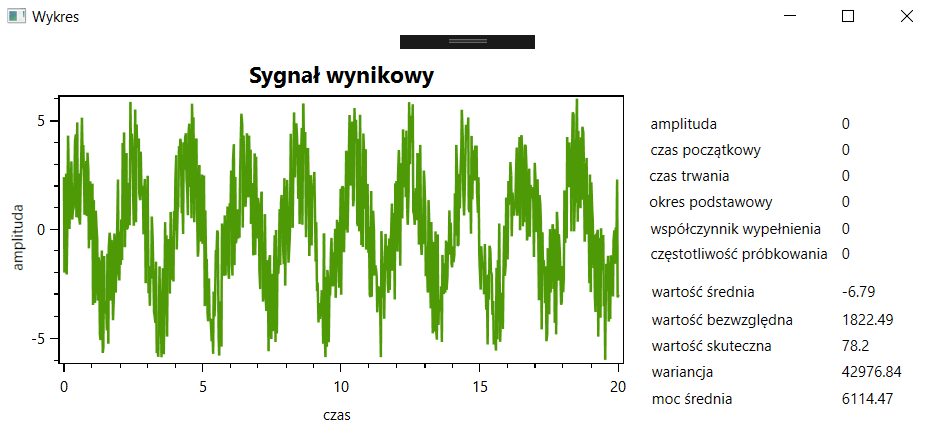
\includegraphics[width=9.3cm]{DodawanieSinRozkA3t120d40h5.png}
 \vspace{-0.3cm}
 \caption{Wykres dla wyników eksperymentu dwunastego}
 \label{Wykres dla wyników eksperymentu dwunastego}
\end{figure}

\subsection{Eksperyment nr 13}

Eksperyment nr 13 - odejmowanie sygnałów

\subsubsection{Założenia}
Aby wykonać operacje na sygnałach, muszą zgadzać się ich parametry.
\\
Parametry: A, T t1, d, kw.

\subsubsection{Przebieg}
Do generacji odejmowania synałów zostały wybrane sygnał sinusoidalny prostowany jednopołówkowo i sygnał trójkątny o jednakowych podanych parametrach:
\addtokomafont{labelinglabel}{\sffamily}

\begin{labeling}{szj}
\item [Amplituda (A):] 5
\item [Czas trwania (t1):] 25 s
\item [Częstotliwość próbkowania (d): ] 50 Hz
\item [Okres podstawowy (T):] 2 s
\end{labeling}

\subsubsection{Rezultat}
Rezultaty przedstawiają zamieszczone poniżej zrzuty ekranu z programu. Wartości liczbowe oraz wykres funkcji amplitudy od czasu przedstawia \ref{Wykres dla wyników eksperymentu trzynastego}.
\begin{figure}[h!]
 \centering
 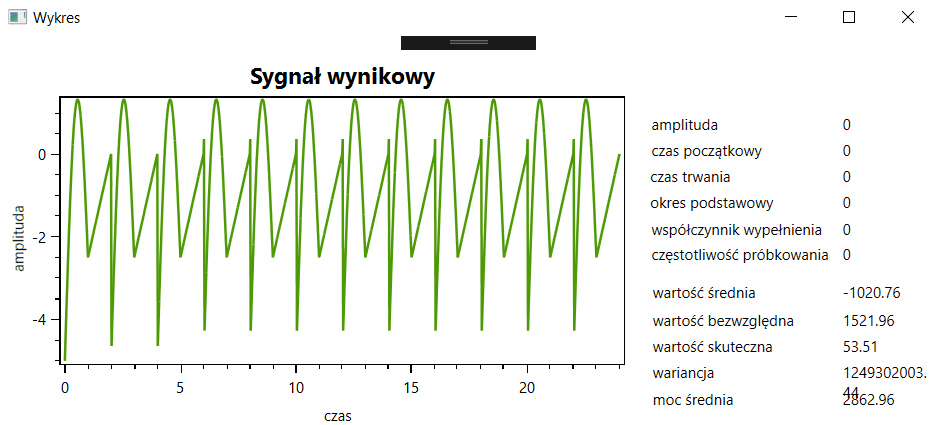
\includegraphics[width=9.3cm]{MinSinJedPTrojA5t125d50T2.png}
 \vspace{-0.3cm}
 \caption{Wykres dla wyników eksperymentu trzynastego}
 \label{Wykres dla wyników eksperymentu trzynastego}
\end{figure}

\subsection{Eksperyment nr 14}

Eksperyment nr 13 - mnożenie sygnałów

\subsubsection{Założenia}
Aby wykonać operacje na sygnałach, muszą zgadzać się ich parametry.

\subsubsection{Przebieg}
Do generacji mnożenia synałów zostały wybrane sygnał sinusoidalny prostowany jednopołówkowo i sygnał trójkątny o jednakowych podanych parametrach:
\addtokomafont{labelinglabel}{\sffamily}

\begin{labeling}{szj}
\item [Amplituda (A):] 5
\item [Czas trwania (t1):] 25 s
\item [Częstotliwość próbkowania (d): ] 50 Hz
\item [Okres podstawowy (T):] 2 s
\end{labeling}

\subsubsection{Rezultat}
Rezultaty przedstawiają zamieszczone poniżej zrzuty ekranu z programu. Wartości liczbowe oraz wykres funkcji amplitudy od czasu przedstawia \ref{Wykres dla wyników eksperymentu czternastego}.
\begin{figure}[h!]
 \centering
 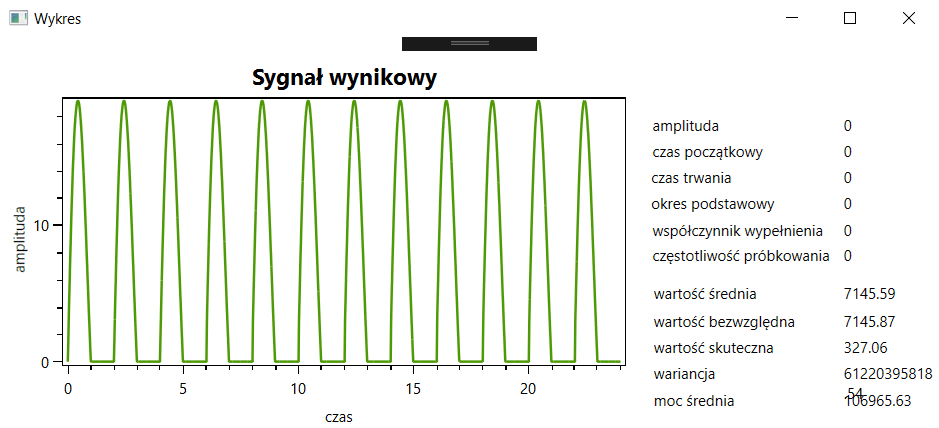
\includegraphics[width=9.3cm]{MnozenieSinJedPTrojA5t125d50T2.png}
 \vspace{-0.3cm}
 \caption{Wykres dla wyników eksperymentu czternastego} 
 \label{Wykres dla wyników eksperymentu czternastego}
\end{figure}

\subsection{Eksperyment nr 15}
\subsubsection{Założenia}
Aby wykonać operacje na sygnałach, muszą zgadzać się ich parametry.

\subsubsection{Przebieg}
Do generacji dzielenia synałów zostały wybrane sygnał o rozkładzie normalnym i sygnał sinusoidalny o jednakowych podanych parametrach:
\addtokomafont{labelinglabel}{\sffamily}

\begin{labeling}{szj}
\item [Amplituda (A):] 3
\item [Czas trwania (t1):] 20 s
\item [Częstotliwość próbkowania (d): ] 40 Hz
\end{labeling}

\subsubsection{Rezultat}
Rezultaty przedstawiają zamieszczone poniżej zrzuty ekranu z programu. Wartości liczbowe oraz wykres funkcji amplitudy od czasu przedstawia \ref{Wykres dla wyników eksperymentu piętnastego}.
\begin{figure}[h!]
 \centering
 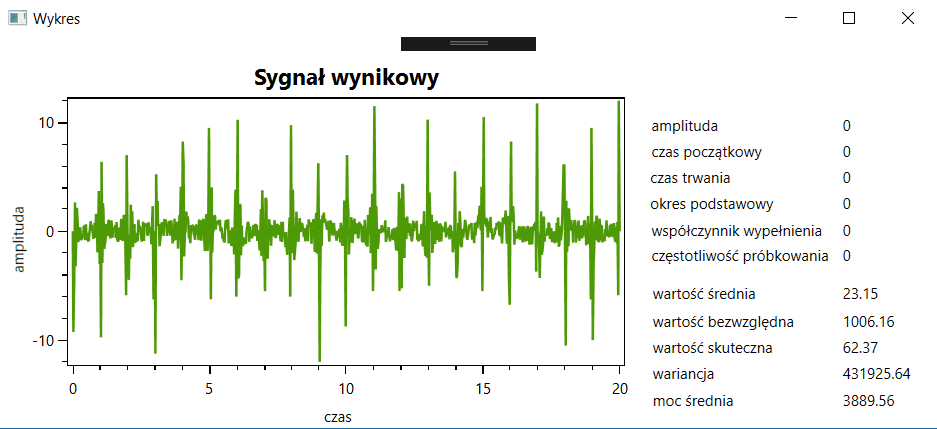
\includegraphics[width=9.3cm]{DzielenieRozkSinA3t120d40h5.png}
 \vspace{-0.3cm}
 \caption{Wykres dla wyników eksperymentu piętnastego}
 \label{Wykres dla wyników eksperymentu piętnastego}
\end{figure}

\section{Wnioski}


Przeprowadzone eksperymenty dowodzą, że  przy małym czasie trwania trzeba zwiekszyć czestotliwosć by gestosć punktów do wykresów byla wystarczajaca - niekoniecznie musi być większa niz czas. Parametr amplitudy ma stosunkowo niewielki wpływ na wygląd graficznej reprezentacji - wykres będzie wyższy lub niższy, ale nie zmienia się jego charakter. Zapimplementowane generatory tworzą bardzo rózne sygnały. 
%%%%%%%%%%%%%%%%%%%%%%%%%%%%%%%%%%%%%%%%%%%%%%%%%%%%%%%%%%%%%%%%%%%%%%%%%%%%%%%%%%%%%%%%%%%%%%%%%%%%%%%%%%%%%%%%%
% PODROZDZIA PT. ZALACZNIKI
%%%%%%%%%%%%%%%%%%%%%%%%%%%%%%%%%%%%%%%%%%%%%%%%%%%%%%%%%%%%%%%%%%%%%%%%%%%%%%%%%%%%%%%%%%%%%%%%%%%%%%%%%%%%%%%%%

\begin{thebibliography}{0}
   \bibitem{l2short} FTIMS Politechnika Łódzka.
    \textsl{Przetwarzanie sygnałów, pojęcia podstawowe Plik}, Wikamp.
 \bibitem{l2short} FTIMS Politechnika Łódzka.
    \textsl{Zadanie 1 Generacja sygnału i szumu}, Wikamp.
\end{thebibliography}




\end{document}
